\lecture{Introduction}{13:00}{26/09/23}{Tamer Elboghdadly}

\section*{Operating Systems}

\begin{itemize}
  \item The Operating System sits inbetween the hardware and application software
  \item It usually is not the actual GUI, but provides functionality for the applications which implement it
  \item OSes typically provide abstractions for applications so that they can run on different hardware
\end{itemize}

\subsection*{User and Kernel Mode}

\begin{itemize}
  \item User mode
  \begin{itemize}
    \item The programs that a user directly interacts with
    \item Uses an API to access hardware, rather than having direct access
  \end{itemize}
  \item Kernel mode
  \begin{itemize}
    \item The programs that run the operating system
    \item Has direct access to hardware
  \end{itemize}
\end{itemize}

\subsection*{System and Application Software}

\begin{itemize}
  \item Application software
  \begin{itemize}
    \item Programs that allow a user to perform a task
    \item Requires the support of system software to run
  \end{itemize}
  \item System software
  \begin{itemize}
    \item Software directly related to the operating system
    \item Manages the boot process
    \item Hardware drivers
    \item File system management
  \end{itemize}
\end{itemize}

\subsection*{The main functions of an Operating System}

\begin{itemize}
  \item Resource management
  \begin{itemize}
    \item Manages the memory, CPU and other hardware to allow multiple programs to run concurrently
    \item Handles requests from applications to allocate more resources
  \end{itemize}
  \item "Extended machine"
  \begin{itemize}
    \item Handles reading and writing to control registers, handlling interrupts, etc
    \item Provides higher level APIs for other software to interact with the hardware
  \end{itemize}
\end{itemize}

\section*{CPU Organisation}

\subsection*{Registers}

\begin{figure}[h]
  \caption{General purpose registers in an x86 Intel CPU}
  \centering
  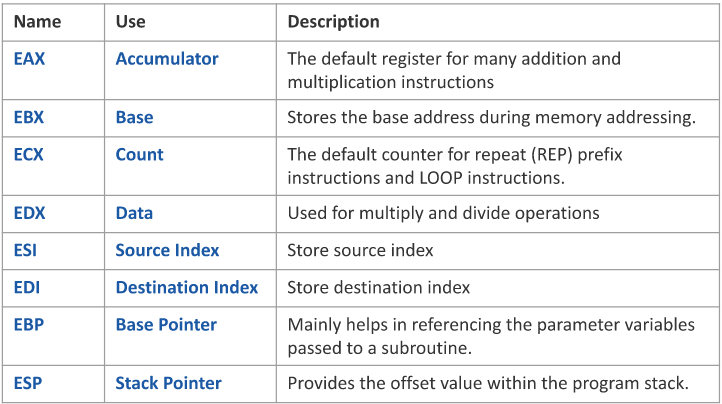
\includegraphics[width=0.8\textwidth]{registers.png}
\end{figure}